\section{Ejercicio 7}

\par Para comprender su funcionamiento comenzamos a hacer pruebas y observamos las salidas entregadas por el scheduler SchedMistery.\\\\

\textbf{Lote de Prueba 1}
\\
\par Como primer caso, utilizamos un lote con seis procesos sin llamadas bloqueantes y con idéntica longitud (cantidad de quantums a consumir). Cuatro de ellos comienzan en el tiempo cero, mientras que los otros dos llegan en el tiempo 50. Esta diferenciación nos servirá para ver si el scheduler les da algún trato diferente a los que llegan. Vamos a pasarle como parámetros los valores `2', `4', `8', `16' y `32' e intentaremos determinar para qué utiliza estos valores.

\begin{figure}[h]
  \centering
    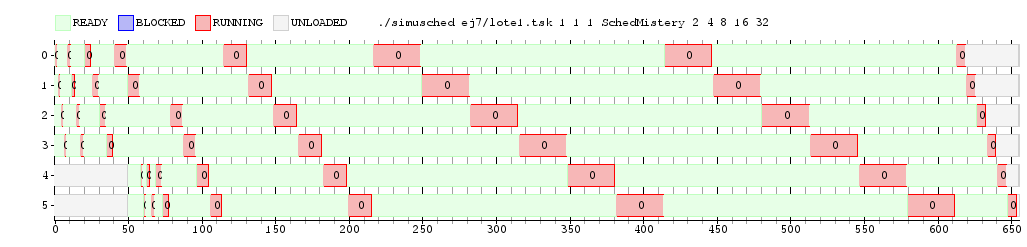
\includegraphics[width=1\textwidth]{images/ej7/lote1.png}
  \label{fig: lote7_1}
\end{figure}

\par En la imagen podemos observar los resultados del primer lote. Lo primero que notamos es que el scheduler tiene un funcionamiento similar al Round Robin, dándole un quantum a cada proceso. Pero estos quantums no tienen siempre la misma longitud. Viendo en detalle los valores vemos que el primer quantum de cada proceso tiene longitud 1, mientras que después toma los valores pasados por parámetro. Con esto podemos insinuar que tiene distintas colas de prioridad: una principal con quantum 1 y luego una por cada parámetro de entrada (con quantum de su valor); y al finalizar su quantum se los mueve a una cola de prioridad menor.
\par Notamos también que al ingresar los dos procesos mas tarde ejecutan sus quantums hasta llegar a la cola de prioridad de los otros cuatro y se posicionan luego de estos. De este detalle podemos determinar que las colas de prioridad son FIFO.
\par Otro detalle es que al llegar a la última cola de prioridad se mantienen en ella. Es algo predecible, pero vale la pena tenerlo en cuenta.\\\\

\textbf{Lote de Prueba 2}
\\
\par Como segundo caso utilizaremos un lote con tres procesos, dos con llamadas bloqueantes y un tercero sin llamadas bloqueantes. Veremos de qué forma se maneja el scheduler con respecto a los procesos con llamadas bloqueantes. Utilizaremos el proceso sin llamadas bloqueantes para comparar los quantums otorgados a cada proceso.

\begin{figure}[h]
  \centering
    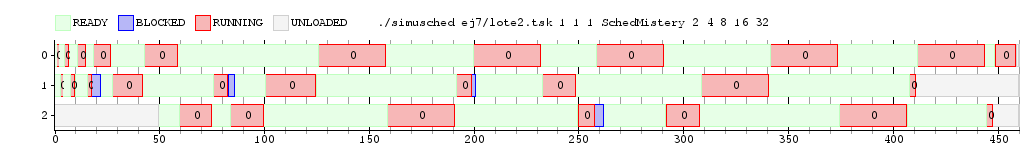
\includegraphics[width=1\textwidth]{images/ej7/lote2.png}
  \label{fig: lote7_2}
\end{figure}

\par En la imagen se observan los resultados del segundo lote. Podemos observar que al regresar de un bloqueo los procesos tienen quantums de diversas longitudes. A simple vista no podemos afirmar nada, así que veremos en detalle los momentos previos y posteriores a las llamadas bloqueantes de cada proceso.

\begin{center}
  \begin{tabular}{ | c | c | c | c | c | }
    \hline
    \textbf{FILA} & \textbf{Proceso} & \textbf{Número de bloqueo} & \textbf{Prioridad al bloquearse} & \textbf{Longitud del próximo quantum} \\ \hline
	\textbf{1} & 1 & 1 & 3 & 14 \\ \hline
  \textbf{2} & 1 & 2 & 5 & 24 \\ \hline
	\textbf{3} & 1 & 3 & 6 & 16 \\ \hline
	\textbf{4} & 2 & 1 & 6 & 16 \\ \hline
  \end{tabular}
\end{center}

\par Vamos a analizar las filas de la tabla para tratar de definir el funcionamiento del scheduler.
\begin{itemize}
	\item En la fila 1 el quantum posterior es de longitud 14: 2 + 4 + 8. Con esto podemos decir que al volver de su bloqueo se lo colocó en la cola de prioridad 2. Al no haber nadie en las cola de prioridad 2, 3 y 4 pudo ejecutar 3 veces seguidas. Luego el scheduler lo colocó al final de la cola de prioridad 5 (detrás del proceso 0). En resumen, el proceso pasó a estado bloqueado luego de estar en la cola de prioridad 3 y al volver de su bloqueo el scheduler lo colocó en la cola de prioridad 2.
	\item En la fila 2 el quantum posterior es de longitud 24: 8 + 16. Con esto podemos decir que el scheduler colocó al proceso en la cola de prioridad 4. Al estar vacías las colas de prioridad 4 y 5 pudo ejecutar dos veces seguidas. Al llegar a la cola de prioridad 6 se posicionó al final (luego del proceso 0). En resumen, el prceso hizo una llamada bloqueante luego de estar en al cola de prioridad 5 y al volver el scheduler lo colocó al final de la cola de prioridad 4.
	\item En la fila 3 el quantum posterior es de longitud 16. con esto podemos decir que el scheduler colocó al proceso en la cola de prioridad 5 (con longitud 16). El proceso ejecutó una vez y luego se colocó al final de la cola de prioridad 6 (luego del proceso 0). En resumen, el proceso realizó una llamada bloqueante luego de estar en la cola de proridad 6 y al volver el scheduler lo colocó en la cola de prioridad 5. Luego de ejecutar su quantum de longitud 16 el scheduler lo colocó en la cola de prioridad 6 (detrás de los procesos 2 y 0).
	\item El caso de la fila 4 es muy similar al de la fila 3. El proceso realizó una llamada bloqueante luego de estar en la cola de prioridad 6 y al volver el scheduler lo colocó al final de la cola de prioridad 5. Ejecutó un quantum de longitud 16 y luego fué colocado al final de la cola de prioridad 6 (detrás de los procesos 1 y 2).
  \item Vale aclarar que no encontramos importancia al número de bloqueo, ya que no notamos cambios con respecto a la primer llamada, la segunda o la i-ésima.
\end{itemize}
\par Viendo en detalle los casos antes listados podemos insinuar que cuando un proceso vuelve de un bloqueo, el scheduler lo coloca al final de la cola de prioridades un número menor a la prioridad que tenía al bloquearse.

\par Luego de correr otros lotes de prueba similares pudimos confirmar las insinuaciones antes listadas y realizamos el scheduler SchedNoMistery que responde a las características del scheduler SchedMistery.
\par No adjuntamos las imágenes salidas de este scheduler porque eran iguales a las del scheduler a copiar y no resultaban relevantes. Estas pruebas pueden reproducirse utilizando el Makefile con el parámetro `ejercicio7'.